% Options for packages loaded elsewhere
% Options for packages loaded elsewhere
\PassOptionsToPackage{unicode}{hyperref}
\PassOptionsToPackage{hyphens}{url}
\PassOptionsToPackage{dvipsnames,svgnames,x11names}{xcolor}
%
\documentclass[
  letterpaper,
  DIV=11,
  numbers=noendperiod]{scrartcl}
\usepackage{xcolor}
\usepackage{amsmath,amssymb}
\setcounter{secnumdepth}{5}
\usepackage{iftex}
\ifPDFTeX
  \usepackage[T1]{fontenc}
  \usepackage[utf8]{inputenc}
  \usepackage{textcomp} % provide euro and other symbols
\else % if luatex or xetex
  \usepackage{unicode-math} % this also loads fontspec
  \defaultfontfeatures{Scale=MatchLowercase}
  \defaultfontfeatures[\rmfamily]{Ligatures=TeX,Scale=1}
\fi
\usepackage{lmodern}
\ifPDFTeX\else
  % xetex/luatex font selection
\fi
% Use upquote if available, for straight quotes in verbatim environments
\IfFileExists{upquote.sty}{\usepackage{upquote}}{}
\IfFileExists{microtype.sty}{% use microtype if available
  \usepackage[]{microtype}
  \UseMicrotypeSet[protrusion]{basicmath} % disable protrusion for tt fonts
}{}
\makeatletter
\@ifundefined{KOMAClassName}{% if non-KOMA class
  \IfFileExists{parskip.sty}{%
    \usepackage{parskip}
  }{% else
    \setlength{\parindent}{0pt}
    \setlength{\parskip}{6pt plus 2pt minus 1pt}}
}{% if KOMA class
  \KOMAoptions{parskip=half}}
\makeatother
% Make \paragraph and \subparagraph free-standing
\makeatletter
\ifx\paragraph\undefined\else
  \let\oldparagraph\paragraph
  \renewcommand{\paragraph}{
    \@ifstar
      \xxxParagraphStar
      \xxxParagraphNoStar
  }
  \newcommand{\xxxParagraphStar}[1]{\oldparagraph*{#1}\mbox{}}
  \newcommand{\xxxParagraphNoStar}[1]{\oldparagraph{#1}\mbox{}}
\fi
\ifx\subparagraph\undefined\else
  \let\oldsubparagraph\subparagraph
  \renewcommand{\subparagraph}{
    \@ifstar
      \xxxSubParagraphStar
      \xxxSubParagraphNoStar
  }
  \newcommand{\xxxSubParagraphStar}[1]{\oldsubparagraph*{#1}\mbox{}}
  \newcommand{\xxxSubParagraphNoStar}[1]{\oldsubparagraph{#1}\mbox{}}
\fi
\makeatother

\usepackage{color}
\usepackage{fancyvrb}
\newcommand{\VerbBar}{|}
\newcommand{\VERB}{\Verb[commandchars=\\\{\}]}
\DefineVerbatimEnvironment{Highlighting}{Verbatim}{commandchars=\\\{\}}
% Add ',fontsize=\small' for more characters per line
\usepackage{framed}
\definecolor{shadecolor}{RGB}{241,243,245}
\newenvironment{Shaded}{\begin{snugshade}}{\end{snugshade}}
\newcommand{\AlertTok}[1]{\textcolor[rgb]{0.68,0.00,0.00}{#1}}
\newcommand{\AnnotationTok}[1]{\textcolor[rgb]{0.37,0.37,0.37}{#1}}
\newcommand{\AttributeTok}[1]{\textcolor[rgb]{0.40,0.45,0.13}{#1}}
\newcommand{\BaseNTok}[1]{\textcolor[rgb]{0.68,0.00,0.00}{#1}}
\newcommand{\BuiltInTok}[1]{\textcolor[rgb]{0.00,0.23,0.31}{#1}}
\newcommand{\CharTok}[1]{\textcolor[rgb]{0.13,0.47,0.30}{#1}}
\newcommand{\CommentTok}[1]{\textcolor[rgb]{0.37,0.37,0.37}{#1}}
\newcommand{\CommentVarTok}[1]{\textcolor[rgb]{0.37,0.37,0.37}{\textit{#1}}}
\newcommand{\ConstantTok}[1]{\textcolor[rgb]{0.56,0.35,0.01}{#1}}
\newcommand{\ControlFlowTok}[1]{\textcolor[rgb]{0.00,0.23,0.31}{\textbf{#1}}}
\newcommand{\DataTypeTok}[1]{\textcolor[rgb]{0.68,0.00,0.00}{#1}}
\newcommand{\DecValTok}[1]{\textcolor[rgb]{0.68,0.00,0.00}{#1}}
\newcommand{\DocumentationTok}[1]{\textcolor[rgb]{0.37,0.37,0.37}{\textit{#1}}}
\newcommand{\ErrorTok}[1]{\textcolor[rgb]{0.68,0.00,0.00}{#1}}
\newcommand{\ExtensionTok}[1]{\textcolor[rgb]{0.00,0.23,0.31}{#1}}
\newcommand{\FloatTok}[1]{\textcolor[rgb]{0.68,0.00,0.00}{#1}}
\newcommand{\FunctionTok}[1]{\textcolor[rgb]{0.28,0.35,0.67}{#1}}
\newcommand{\ImportTok}[1]{\textcolor[rgb]{0.00,0.46,0.62}{#1}}
\newcommand{\InformationTok}[1]{\textcolor[rgb]{0.37,0.37,0.37}{#1}}
\newcommand{\KeywordTok}[1]{\textcolor[rgb]{0.00,0.23,0.31}{\textbf{#1}}}
\newcommand{\NormalTok}[1]{\textcolor[rgb]{0.00,0.23,0.31}{#1}}
\newcommand{\OperatorTok}[1]{\textcolor[rgb]{0.37,0.37,0.37}{#1}}
\newcommand{\OtherTok}[1]{\textcolor[rgb]{0.00,0.23,0.31}{#1}}
\newcommand{\PreprocessorTok}[1]{\textcolor[rgb]{0.68,0.00,0.00}{#1}}
\newcommand{\RegionMarkerTok}[1]{\textcolor[rgb]{0.00,0.23,0.31}{#1}}
\newcommand{\SpecialCharTok}[1]{\textcolor[rgb]{0.37,0.37,0.37}{#1}}
\newcommand{\SpecialStringTok}[1]{\textcolor[rgb]{0.13,0.47,0.30}{#1}}
\newcommand{\StringTok}[1]{\textcolor[rgb]{0.13,0.47,0.30}{#1}}
\newcommand{\VariableTok}[1]{\textcolor[rgb]{0.07,0.07,0.07}{#1}}
\newcommand{\VerbatimStringTok}[1]{\textcolor[rgb]{0.13,0.47,0.30}{#1}}
\newcommand{\WarningTok}[1]{\textcolor[rgb]{0.37,0.37,0.37}{\textit{#1}}}

\usepackage{longtable,booktabs,array}
\usepackage{calc} % for calculating minipage widths
% Correct order of tables after \paragraph or \subparagraph
\usepackage{etoolbox}
\makeatletter
\patchcmd\longtable{\par}{\if@noskipsec\mbox{}\fi\par}{}{}
\makeatother
% Allow footnotes in longtable head/foot
\IfFileExists{footnotehyper.sty}{\usepackage{footnotehyper}}{\usepackage{footnote}}
\makesavenoteenv{longtable}
\usepackage{graphicx}
\makeatletter
\newsavebox\pandoc@box
\newcommand*\pandocbounded[1]{% scales image to fit in text height/width
  \sbox\pandoc@box{#1}%
  \Gscale@div\@tempa{\textheight}{\dimexpr\ht\pandoc@box+\dp\pandoc@box\relax}%
  \Gscale@div\@tempb{\linewidth}{\wd\pandoc@box}%
  \ifdim\@tempb\p@<\@tempa\p@\let\@tempa\@tempb\fi% select the smaller of both
  \ifdim\@tempa\p@<\p@\scalebox{\@tempa}{\usebox\pandoc@box}%
  \else\usebox{\pandoc@box}%
  \fi%
}
% Set default figure placement to htbp
\def\fps@figure{htbp}
\makeatother

\ifLuaTeX
  \usepackage{luacolor}
  \usepackage[soul]{lua-ul}
\else
  \usepackage{soul}
\fi




\setlength{\emergencystretch}{3em} % prevent overfull lines

\providecommand{\tightlist}{%
  \setlength{\itemsep}{0pt}\setlength{\parskip}{0pt}}



 


\KOMAoption{captions}{tableheading}
\makeatletter
\@ifpackageloaded{caption}{}{\usepackage{caption}}
\AtBeginDocument{%
\ifdefined\contentsname
  \renewcommand*\contentsname{Table of contents}
\else
  \newcommand\contentsname{Table of contents}
\fi
\ifdefined\listfigurename
  \renewcommand*\listfigurename{List of Figures}
\else
  \newcommand\listfigurename{List of Figures}
\fi
\ifdefined\listtablename
  \renewcommand*\listtablename{List of Tables}
\else
  \newcommand\listtablename{List of Tables}
\fi
\ifdefined\figurename
  \renewcommand*\figurename{Figure}
\else
  \newcommand\figurename{Figure}
\fi
\ifdefined\tablename
  \renewcommand*\tablename{Table}
\else
  \newcommand\tablename{Table}
\fi
}
\@ifpackageloaded{float}{}{\usepackage{float}}
\floatstyle{ruled}
\@ifundefined{c@chapter}{\newfloat{codelisting}{h}{lop}}{\newfloat{codelisting}{h}{lop}[chapter]}
\floatname{codelisting}{Listing}
\newcommand*\listoflistings{\listof{codelisting}{List of Listings}}
\makeatother
\makeatletter
\makeatother
\makeatletter
\@ifpackageloaded{caption}{}{\usepackage{caption}}
\@ifpackageloaded{subcaption}{}{\usepackage{subcaption}}
\makeatother
\usepackage{bookmark}
\IfFileExists{xurl.sty}{\usepackage{xurl}}{} % add URL line breaks if available
\urlstyle{same}
\hypersetup{
  pdftitle={How did Ivory Coast win AFCON 2023 despite sacking their manager during the Tournament, and was it deserved?},
  pdfauthor={Your Name (Student ID)},
  colorlinks=true,
  linkcolor={blue},
  filecolor={Maroon},
  citecolor={Blue},
  urlcolor={Blue},
  pdfcreator={LaTeX via pandoc}}


\title{How did Ivory Coast win AFCON 2023 despite sacking their manager
during the Tournament, and was it deserved?}
\author{Your Name (Student ID)}
\date{2026-05-12}
\begin{document}
\maketitle

\renewcommand*\contentsname{Table of contents}
{
\hypersetup{linkcolor=}
\setcounter{tocdepth}{3}
\tableofcontents
}

\section{My Resources}\label{my-resources}

\textbf{Live dashboard:}
\url{https://YOUR-USERNAME.github.io/nba-analytics/}

\textbf{Repository:}
\url{https://github.com/YOUR-USERNAME/nba-analytics}\\

\section{\texorpdfstring{\ul{1.
Introduction}}{1. Introduction}}\label{introduction}

AFCON 2023 was hosted in Côte d'Ivoire (Ivory Coast), and it saw the
hosts lift the title. This victory was remarkable not just because it
was a home tournament, but the team were on the brink of elimination
during the group stage. After their win in the first game, Ivory Coast
followed that by losing two consecutive games to Nigeria and Equatorial
Guinea which saw them finish in 3rd place, narrowly qualifying due to
them being the 4th best 3rd place finishers. Due to this failure in the
group stage, the Ivorian Football Federation took the decision to sack
the head coach Jean-Louis Gasset and replace him with Emerese Faé, who
was the Ivory Coast under 23 coach.

Following this there was an unexpected revival, with Ivory Coast which
led to AFCON victory. Faé's side beat Senegal in the Round of 16, Mali
in the Quarter Final, Democratic Republic of Congo in the Semi Final,
and then defeated Nigeria in the final, which was one of the team's that
they had previously lost to in the group stage. They didn't only just
beat them, they beat them convincingly as they dominated the final. The
transformation between the two managers was visible, but the question
that this report seeks to answer is whether the data supports the
outcome: How did Ivory Coast win AFCON 2023 despite sacking their
manager during the Tournament, and was it deserved?

The question is interesting because football tournaments can be won due
to pure luck and individual brilliance whilst also posting poor
underlying numbers. On the contrast, a dominant team can lose to a
single moment . Expected Goals (xG), defensive action metrics, attacking
metrics and shot quality data offers a way to cut through the narrative
and allows us to analyse what exactly is happening with the players on
the pitch.

The dashboard and the accompanying analysis is structured around the
comparison between the group stage performance under Jean-Louis Gasset
and the Knockout Stage performance under Emerese Faé, which individual
players drove the improvement, and underlying data suggesting whether
the title was deserved. The data that has been used throughout this
report was sourced from StatsBomb's open data repository, which has
provided event-level data for the AFCON data. The dashboard is hosted
publicly on GitHub Pages and built using R, ggplot2 and Plotly, with the
full code available in the repository that has been linked.

\section{\texorpdfstring{\ul{2. Data Collection and
Preparation}}{2. Data Collection and Preparation}}\label{data-collection-and-preparation}

\subsection{\texorpdfstring{\ul{2.1 Data
Source}}{2.1 Data Source}}\label{data-source}

All the data that has been used in the analysis was obtained from
StatBomb's open data repository, which was computed into R via the
statsbombr package (STATSBOMB REFERENCE). This open data provided event
level match data for AFCON, which allowed for extensive game by game
analysis to be conducted.

The StatsBomb event data model captures every on the ball action in a
match as its own event, each with a timestamp, location (expressed as an
x,y coordinate on a 120 x 80 pitch), the player and the possession team
involved, and many more action specific events.

\section{\texorpdfstring{\ul{4. Findings}}{4. Findings}}\label{findings}

\subsection{\texorpdfstring{\ul{4.1 Tournament Overview and the Group
Stage
Struggle}}{4.1 Tournament Overview and the Group Stage Struggle}}\label{tournament-overview-and-the-group-stage-struggle}

Across the whole tournament, Ivory Coast played 7 matches, winning 4,
drawing one (won the game via a penalty shootout) and losing twice.
Their two defeats came in the group stage where they lost to Nigeria 1-0
and Equatorial Guinea 4-0 in the final group stage game, which triggered
the managerial change. During the knockout stages, Ivory Coast won three
games and drew one, which they won on penalties. They had performed at a
much higher standard, and that will be analysed later in this section.
Table x summarises Ivory Coast's full tournament timeline, showing who
they had faced, what the score was and what the result of the game was.

\begin{verbatim}
  competition_stage.name          opponent ivc_score opp_score result
1                  Final           Nigeria         2         1    Win
2            Semi-finals          Congo DR         1         0    Win
3            Round of 16           Senegal         1         1   Draw
4         Quarter-finals              Mali         2         1    Win
5            Group Stage Equatorial Guinea         0         4   Loss
6            Group Stage           Nigeria         0         1   Loss
7            Group Stage     Guinea-Bissau         2         0    Win
\end{verbatim}

The underlying data from these matches tell us a different story. As
shown in Figure 1, Ivory Coast had a steady accumulation of xG in the
group stage. Across the entire group stage, they accumulated 3.39 xG per
game, which comes to an average of 1.13 per game. Taking the results
into consideration, we can see that they produced inconsistent
performances throughout the group stage, with the two defeats. Despite
losing 4-0 in the last game to Equatorial Guinea, the team had generated
2.06 xG, which is more than the first two games combined. The lack of xG
within those first two games indicate a lack of attacking creativity and
a difficulty in producing high quality opportunities. However in the
last game of the group stage, despite the result, they managed to create
the chances but were not able to finish them off. This sharp defeat led
to the managerial change, even though they narrowly progressed to the
next stage.

\begin{Shaded}
\begin{Highlighting}[]
\FunctionTok{readRDS}\NormalTok{(}\StringTok{"cuumulative\_ivorycoast\_xgplot.rds"}\NormalTok{)}
\end{Highlighting}
\end{Shaded}

\pandocbounded{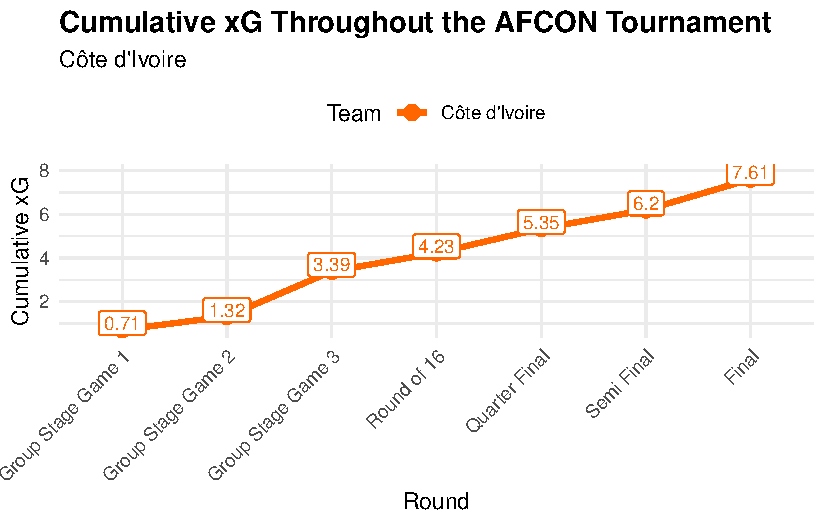
\includegraphics[keepaspectratio]{MAINASSIGNMENT_files/figure-pdf/unnamed-chunk-1-1.pdf}}

\subsection{\texorpdfstring{\ul{4.2 The Managerial Change: The
introduction of Emerse
Faé}}{4.2 The Managerial Change: The introduction of Emerse Faé}}\label{the-managerial-change-the-introduction-of-emerse-fauxe9}

The appointment of Emerse Faé was a surprise for many reasons. No one
expected a team to dismiss their manager during the season, especially
as they had reached the knockout stages. However, the performances from
the team under head coach Jean-Louis Gasset caused for immediate change.
The managerial change produced measurable data evidenced changes across
all metrics of Ivory Coast's performance. An examination of six areas of
comparison between the two managers will best highlight the significant
impact that the new manager created.

\subsubsection{\texorpdfstring{\ul{Shot Map and Attacking
Locations}}{Shot Map and Attacking Locations}}\label{shot-map-and-attacking-locations}

The shot maps in Figure 2 offer the clearest immediate illustration of
how the team's attacking intent had changed.

Under Emerse Faé, Ivory Coast's shots appear to be more centrally
concentrated inside and around the penalty area. a large proportion of
these shots came in a dangerous area, which therefore gave them a higher
chance of scoring. This suggests that there was a more direct attacking
structure, which was focused on creating higher quality opportunities in
central areas for their attackers. Even the long range attempts from
outside the box are a t

In contrast,

\begin{Shaded}
\begin{Highlighting}[]
\FunctionTok{readRDS}\NormalTok{(}\StringTok{"manager\_comparison\_shotmap.rds"}\NormalTok{)}
\end{Highlighting}
\end{Shaded}

\pandocbounded{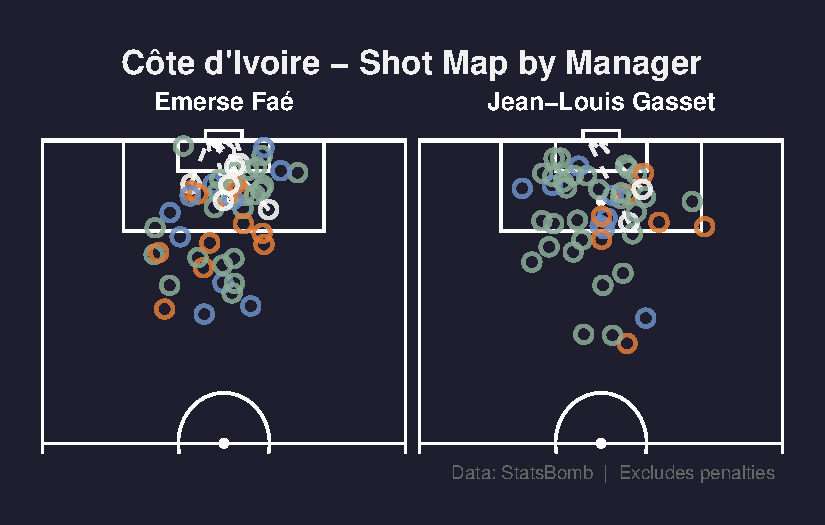
\includegraphics[keepaspectratio]{MAINASSIGNMENT_files/figure-pdf/unnamed-chunk-2-1.pdf}}

\section{References}\label{references}




\end{document}
